\section{Comunicación vehicular}\label{section:comunicacion_vehicular}
Los RSU y OBU son los encargados de proveer las posiciones de los vehículos a motor de la \emph{Nube de Conductores}. El OBU se encuentra integrado en el vehículo, y envía a través de \emph{IEEE 802.11p} las posiciones de los vehículos a la RSU. La RSU recoge los datos enviados por la OBU y los retransmite a la nube, al igual que recibe datos de la nube y los retransmite al OBU.

\subsection{Unidad en carretera}\label{subsection:unidad_carretera}
Formato por un router que se comunica a través de \emph{IEEE 802.11p}, y un computador conectado tanto al router como a una red LTE. Actúan como puente entre las OBU instaladas en los vehículos y la nube. El RSU escucha y escribe a través de dos canales:
\begin{enumerate}
	\item En el canal LTE recibe los mensajes HTTP/1.1 que provienen de la Nube de Conductores, así como envía las posiciones de los vehículos a la nube. Un Servicio web posibilita la gestión de estos mensajes; el formato es el mismo que el explicado en la sección \ref{ssection:FormatoMensajesNC}.
		
	\item Escucha el canal IEEE 802.11p los mensajes que son enviados por los vehículos, y los redirige a la nube a través de mensajes HTTP/1.1.
\end{enumerate}

\subsubsection{Funcionamiento}
\begin{enumerate}
	\item Se comprueba que el formato del mensaje es correcto. Si no lo es, se descarta.
	\item Lectura del campo \"TYPE\" del mensaje. Dependiendo de su contenido se aplica un proceso diferente: el mensaje puede ser retransmitido a través de Broadcast, se puede mostrar una notificación en un panel informativo en carretera...
\end{enumerate}
		
Una propuesta para añadir funciones adicionales consiste en conectar el RSU a elementos informáticos que pueden existir en la carretera, por ejemplo los paneles informativos, y al enviar un mensaje desde la Nube de Conductores a una RSU en concreto se muestra la información deseada.

\subsection{Unidad en el vehículo}
Dentro del ecosistema vehicular existen varias unidades con diferentes papeles: el OBU, el HMI (Human-Machine interface) y la interfaz OpenXC (o tecnología equivalente). Para darse la comunicación con todas las plataformas se depende de la existencia de RSU desplegadas en la carretera.

\subsubsection{OBU}
Formado por un router que se comunica a través de IEEE 802.11p, un dispositivo GPS conectado al router, y un computador conectado al router a través de un conector RJ-45. A traves de esta red se reciben mensajes de diferentes RSU que se encuentran desplegadas en la carretera, al igual que se envían mensajes informando sobre la posición del vehículo a través de Broadcast. Su funcionamiento consiste en:
\begin{itemize}
	\item Obtener la posición del vehículo realizando peticiones al router.
	\item Mandar periódicamente las posiciones a través de broadcast.
	\item Escuchar los mensajes que mandan las RSU.
	\item Ofrecer y proveer al usuario la información de los mensajes a través del HMI.
\end{itemize}
	
\subsubsection{Información al usuario}
Para proveer información al conductor se emplea el HMI, el cual consiste en un ordenador de a bordo que contiene diferentes apps. adicionalmente, se puede conectar al OBDII (On-Board Diagnostic)\footnote{Se trata del sistema de diagnóstico del vehículo. Provee información sobre el estado de los diferentes subsistemas del vehículo.} a través de un puerto RS 232 para obtener información del vehículo; como por ejemplo, el estado de los neumáticos.
	
Se ha desarrollado una aplicación conectada por Bluetooth al OBU con la que se muestra al vehículo un mapa con las posiciones de los ciclistas cercanos [Imagen \ref{figure:HMI}]. Cuando un vehículo se acerca a un ciclista o grupo de ciclistas una notificación salta para informar al conductor. Las posiciones de los ciclistas son obtenidas a través de la nube, y almacenadas en el vehículo durante un período de 30 segundos; según llegan las nuevas posiciones desde la nube, se van actualizando. Pasado ese tiempo, los registros que no hayan sido refrescados son eliminados, ya que esto significaría que los nodos han dejado de transmitir.
	
\begin{figure}[H]
	\begin{center}
	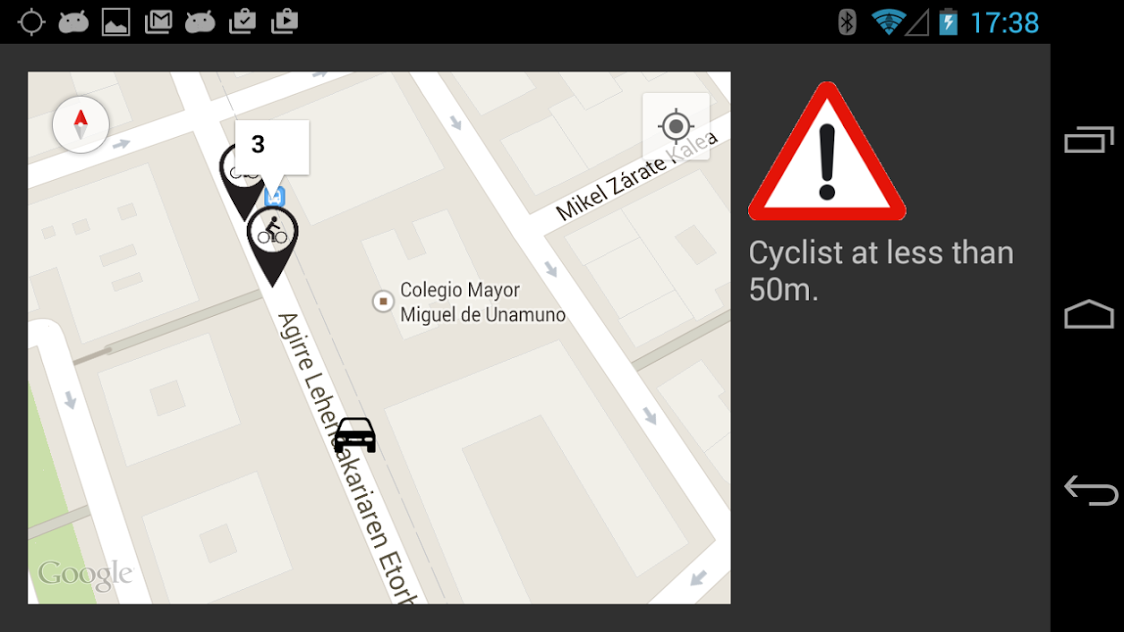
\includegraphics[scale=0.4]{HMI}
	\caption{UI de la aplicación instalada en el HMI}
	\label{figure:HMI}
\end{center}
\end{figure}
	
\subsubsection{Comunicación HMI-OBU}
Para crear el servidor Bluetooth que envíe los mensajes recibidos por el OBU a la aplicación instalada en el HMI, se ha utilizado la librería Bluecove. En el \ref{alg:puntoAccesoHMI_OBU} se abre un punto de acceso para clientes Bluetooth, y se envían los mensajes que se han recibido en el OBU y deben ser mostrados al usuario.

\begin{listing}
	\begin{minipage}{.4\textwidth}
		\begin{minted}[linenos=true]{java}
BluetoothServer server;
StreamConnection cnn;
BufferedWriter writer;
final String UUID = "btspp://localhost:432814212fd123e;name=obu";
StreamConnectionNotifier notifier;
					
// 1. Para que el HMI pueda conectarse al OBU la conexión primero se debe hacer
// visible bajo un UUID determinado.
LocalDevice.getLocalDevice().setDiscoverable(DiscoveryAgent.GIAC);
cnn = notifier.acceptAndOpen();					
					
// 2. Se espera a que un cliente se conecte al servicio Bluetooth
writer = new BufferedWriter(new OutputStreamWriter(cnn.openDataOutputStream()));
					
// 3. Una vez conectado, se envían mensajes al cliente en cuanto son recibidos, mediante
// una cola de mensajes
[...]
					
// 4. Se cierra el socket al finalizar la conexión
writer.close();
cnn.close();
		\end{minted}
	\end{minipage}
\caption{Creación de un punto de acceso Bluetooth en el OBU}\label{alg:puntoAccesoHMI_OBU}
\end{listing}
